\part{虚拟化部分}
\label{part:virtualization}

虚拟化的主要目标是在一台主机上运行多个操作系统,以便充分利用大型机上昂
贵的计算资源。随着x86处理器的性能提升以及应用的普及,虚拟化技术的发展也
开始进入到x86架构领域。特别是到20世纪90年代末期,VMware等虚拟化软件厂商
为x86平台上虚拟化技术应用开辟了道路,提供了以VMM(Virtual Machine
  Monitor)为中心,对PC服务器平台虚拟化的软件解决方案。纯软件解决方案在
性能方面的瓶颈后来又进一步催生出了半虚拟化技术和硬件虚拟化技术,最终
Intel的VT(Virtualization Technology,虚拟化技术)和AMD的SVM(Secure
  Virtual Machine,安全虚拟机)技术均在硬件级提供了对虚拟化的支持。虚拟
化技术被列为2009年度最值得关注的IT技术之首,足可见虚拟化技术在目前企业
计算和应用领域的重要性。

\chapter{KVM}
\label{chap:kvm}

KVM(Kernel-based Virtual Machin)的简称)是一个开源的系统虚拟化模块,
自Linux 2.6.20之后集成在Linux的各个主要发行版本中。它使用Linux自身的调
度器进行管理,所以相对于Xen,其核心源码很少。KVM目前已成为学术界的主
流VMM之一。

\section{关于KVM}
\label{sec:AboutKVM}

\section{安装前的准备工作}
\label{sec:kvmPrepare}

测试环境为:

安装EPEL源

\chapter{Docker}

\section{关于Docker}

Docker是一个开源的应用容器引擎,让开发者可以打包他们的应用以及依赖包到
一个可移植的容器中,然后发布到任何流行的 Linux 机器上,也可以实现虚拟化。
容器是完全使用沙箱机制,相互之间不会有任何接口。几乎没有性能开销,可以
很容易地在机器和数据中心中运行。最重要的是,他们不依赖于任何语言、框架
包括系统。

\begin{verbatim}
sudo apt-get install git
sudo apt-get install git-core
\end{verbatim}

\section{容器 VS. 虚拟机}

容器为应用程序提供了隔离的运行空间:每个容器内都包含一个独享的完整用户
环境空间,并且一个容器内的变动不会影响其他容器的运行环境,如
图\ref{fig:container}所示。为了能达到这种效果,容器技术使用了一系
列的系统级别的机制诸如利用Linux namespaces来进行空间隔离,通过文件系统
的挂载点来决定容器可以访问哪些文件,通过cgroups来确定每个容器可以利用多
少资源。此外容器之间共享同一个系统内核,这样当同一个库被多个容器使用时,
内存的使用效率会得到提升。

\begin{figure}[!htbp]
  \centering
  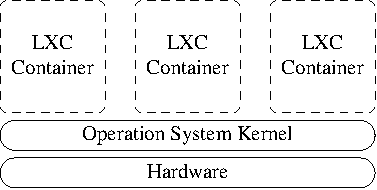
\includegraphics{graph/container01.pdf}
    \caption{容器架构模型}
  \label{fig:container}
\end{figure}

对于系统虚拟化技术来说,虚拟层为用户提供了一个完整的虚拟机:包括内核在
内的一个完整的系统镜像。CPU虚拟化技术可以为每个用户提供一个独享且和其他
用户隔离的系统环境,虚拟层可以为每个用户分配虚拟化后的CPU、内存和IO设备
资源,如图\ref{fig:virtualization}所示。

\begin{figure}[!htbp]
  \centering
  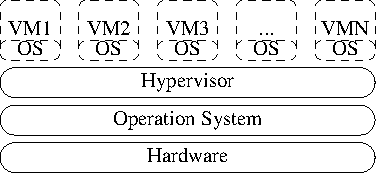
\includegraphics{graph/virtualization01.pdf}
    \caption{虚拟化架构模型}
  \label{fig:virtualization}
\end{figure}

\begin{verbatim}
git config --global user.name "Laven Liu"
git config --global user.email "air.man.six@gmail.com"
\end{verbatim}

\section{安装Docker}

\begin{verbatim}
# yum install docker-io
# service docker start
\end{verbatim}

\begin{figure}[hbtp]
  \centering
  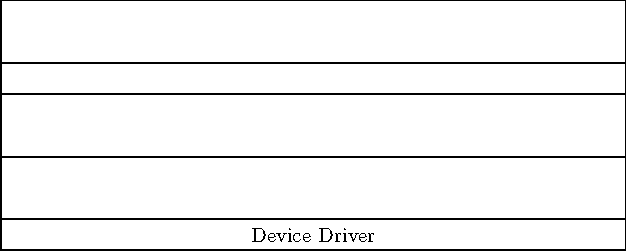
\includegraphics{graph/os-arch-mps.pdf}
    \caption{系统架构}
  \label{fig:OSArch}
\end{figure}
